% !TEX program = xelatex
\documentclass[a4paper,10pt]{article}

\makeatletter
\let\@expl@@@mark@update@singlecol@structures@@\relax
\makeatother

\usepackage[a4paper, left=1.0cm, right=1.0cm, top=0.90cm, bottom=1.05cm, footskip=0.48cm]{geometry}
\usepackage{fontspec}
\usepackage{amsmath, amssymb}
\usepackage{array, colortbl}
\usepackage[table]{xcolor}
\usepackage{tcolorbox}
\tcbuselibrary{skins, breakable}
\usepackage{fancyhdr}
\usepackage{enumitem}
\usepackage{tikz}
\usetikzlibrary{calc, angles, quotes, arrows.meta, decorations.markings}

\makeatletter
\newcommand{\NGSFindFonts}{%
  \IfFileExists{../../../fonts/KhmerOSsiemreap.ttf}{%
    \def\NGSUserPath{../../../fonts/}\def\NGSSysPath{../../../fonts/}%
  }{%
    \IfFileExists{../../../../fonts/KhmerOSsiemreap.ttf}{%
      \def\NGSUserPath{../../../../fonts/}\def\NGSSysPath{../../../../fonts/}%
    }{%
      \IfFileExists{fonts/KhmerOSsiemreap.ttf}{%
        \def\NGSUserPath{fonts/}\def\NGSSysPath{fonts/}%
      }{%
        \def\NGSUserPath{C:/Users/user/AppData/Local/Microsoft/Windows/Fonts/}%
        \def\NGSSysPath{C:/Windows/Fonts/}%
      }%
    }%
  }%
}
\NGSFindFonts
\makeatother

\XeTeXlinebreaklocale "km"
\XeTeXlinebreakskip = 0pt plus 1pt minus 0.1pt

\setmainfont[
  Path = {\NGSUserPath},
  Extension = .ttf,
  UprightFont = KhmerOSsiemreap,
  BoldFont = KhmerOSsiemreap,
  BoldFeatures = {FakeBold=1.8},
  ItalicFont = KhmerOSsiemreap,
  ItalicFeatures = {FakeSlant=0.25}
]{KhmerOSsiemreap}

\newfontfamily\muol[Path={\NGSUserPath}]{KhmerOSmuollight.ttf}
\newfontfamily\enfont[Path={\NGSSysPath}, Scale=1.0]{times.ttf}
\newfontfamily\enbold[Path={\NGSSysPath}, Scale=1.0]{timesbd.ttf}
\newfontfamily\calibrifont[Path={\NGSSysPath}, Scale=0.95]{calibri.ttf}

\DeclareTextFontCommand{\en}{\enfont}
\newcommand{\enbf}[1]{{\enbold #1}}

\definecolor{headgray}{HTML}{E2E2E2}
\definecolor{panelgray}{HTML}{F5F5F5}

\pagestyle{fancy}
\fancyhf{}
\renewcommand{\headrulewidth}{0pt}
\renewcommand{\footrulewidth}{0.4pt}
\fancyfoot[L]{\rule{0pt}{11pt}\fontsize{8.5pt}{11pt}\selectfont អនុវិទ្យាល័យព្រះក្រសាំង $\;\vert\;$ គណិតវិទ្យា ថ្នាក់ទី៨ $\;\vert\;$ មេរៀនទី១៤ (១៤.៣) ផ្ទៃក្រឡាចតុកោណព្នាយ}
\fancyfoot[R]{\rule{0pt}{11pt}\fontsize{8.5pt}{11pt}\selectfont ទំព័រ \en{\thepage\,/\,2}}

\setlength{\parindent}{0pt}
\setlength{\tabcolsep}{4pt}

\newcommand{\tri}[1]{\triangle #1}
\newcommand{\unit}[1]{\,\text{\en{#1}}}
\newcommand{\blank}[1]{\leavevmode\hbox to #1{\dotfill}}
\newcommand{\chkbox}{\tikz[baseline=0.2ex]\draw[black, line width=0.7pt] (0,0) rectangle (1.55ex,1.55ex);}
\newcommand{\cnum}[1]{\tikz[baseline=-0.58ex]\node[circle, fill=black, text=white, inner sep=0.85pt, minimum size=1.95ex, font=\enbold\scriptsize]{#1};}

\newcommand{\rightbox}[4][0.20cm]{%
  \coordinate (rbA) at ($(#3)!#1!(#2)$);
  \coordinate (rbB) at ($(#3)!#1!(#4)$);
  \coordinate (rbC) at ($(rbA)+(#3)!#1!(#4)-(#3)$);
  \draw[black, line width=0.65pt] (rbA) -- (rbC) -- (rbB);
}

\newcommand{\secbar}[2]{%
  \vspace{2.5pt}%
  \begin{tcolorbox}[
    enhanced, sharp corners, colback=headgray, colframe=black,
    boxrule=0.85pt, left=6pt, right=6pt, top=2.5pt, bottom=2.5pt, after skip=3.5pt
  ]
    {\muol\fontsize{9.5pt}{14pt}\selectfont #1}\hfill{\fontsize{9pt}{13pt}\selectfont\textbf{#2}}
  \end{tcolorbox}%
}

\begin{document}
\fontsize{9.6pt}{14.2pt}\selectfont

% ==================== ក្បាលសន្លឹកកិច្ចការ ====================
\begin{tcolorbox}[
  enhanced, sharp corners, colback=white, colframe=black,
  boxrule=1.1pt, left=6pt, right=6pt, top=3.5pt, bottom=3.5pt, after skip=3pt
]
  \begin{minipage}[c]{11.4cm}
    {\muol\fontsize{10.5pt}{15.5pt}\selectfont សន្លឹកកិច្ចការសិស្ស — មេរៀនទី១៤ ៖ ផ្ទៃក្រឡាពហុកោណ}\\[1.5pt]
    \textbf{ចំណុចទី ៣ ៖ ផ្ទៃក្រឡាចតុកោណព្នាយ} (សៀវភៅសិក្សាគោល ទំ.១៩១--១៩៣)
  \end{minipage}\hfill
  \begin{minipage}[c]{7.0cm}
    ឈ្មោះសិស្ស៖ \blank{4.7cm}\\[2pt]
    ថ្នាក់ទី៨៖ \blank{1.4cm} \hspace{0.2cm} ដៃគូទី៖ \blank{2.2cm}
  \end{minipage}
\end{tcolorbox}

% ==================== ផ្នែកទី ១ ៖ E1 - ENGAGE ====================
\secbar{ផ្នែកទី ១ ៖ បេសកកម្មភ្ជាប់បញ្ហា (\enbf{E1}) — ប្រៀបធៀបប្លង់ដីកសិដ្ឋាន \enbf{A} និង \enbf{B}}{\en{3} នាទី (ទស្សន៍ទាយមុនរៀន)}

\begin{tcolorbox}[
  enhanced, sharp corners, colback=panelgray, colframe=black,
  boxrule=0.8pt, left=6pt, right=6pt, top=3pt, bottom=3pt, after skip=3pt
]
  \begin{minipage}[c]{11.3cm}
    ប្លង់ដីនៃកសិដ្ឋានមួយត្រូវបានបែងចែកដោយរបងត្រង់ឈរជាពីរប្លង់ដីរាងចតុកោណព្នាយ $A$ និង $B$ (ទំ.១៩២)៖
    \begin{itemize}[leftmargin=1.2em, itemsep=1pt, topsep=1pt]
      \item \textbf{ប្លង់ដី $A$៖} មានជ្រុងស្របបញ្ឈរ $150\unit{m}$ និង $126\unit{m}$ ហើយទទឹងកែង $120\unit{m}$។
      \item \textbf{ប្លង់ដី $B$៖} មានជ្រុងស្របបញ្ឈរ $126\unit{m}$ និង $100\unit{m}$ ប៉ុន្តែមានទទឹងកែងវែងជាង គឺ $130\unit{m}$។
    \end{itemize}
    \textbf{ទស្សន៍ទាយមុនរៀន៖} \hspace{0.15cm}
    \chkbox\ ប្លង់ $A$ ធំជាង \hspace{0.35cm}
    \chkbox\ ប្លង់ $B$ ធំជាង \hspace{0.35cm}
    \chkbox\ ស្មើគ្នា \hspace{0.35cm}
    \chkbox\ មិនទាន់ប្រាកដ
  \end{minipage}\hfill
  \begin{minipage}[c]{7.0cm}
    \centering
    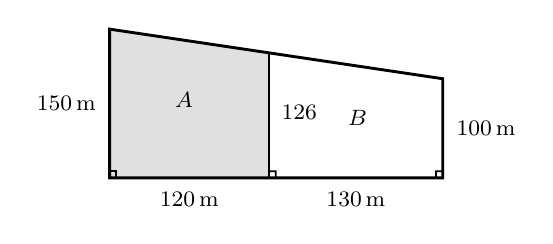
\begin{tikzpicture}[scale=0.45, every node/.style={font=\footnotesize, text=black}]
      \coordinate (P1) at (0,0);
      \coordinate (P2) at (4.5,0);
      \coordinate (P3) at (9.4,0);
      \coordinate (Q1) at (0,4.2);
      \coordinate (Q2) at (4.5,3.52);
      \coordinate (Q3) at (9.4,2.8);
      \fill[gray!24] (P1)--(P2)--(Q2)--(Q1)--cycle;
      \fill[white] (P2)--(P3)--(Q3)--(Q2)--cycle;
      \draw[black, line width=1.05pt] (P1)--(P3)--(Q3)--(Q1)--cycle;
      \draw[black, line width=0.95pt] (P2)--(Q2);
      \rightbox[0.19cm]{Q1}{P1}{P2}
      \rightbox[0.19cm]{Q2}{P2}{P3}
      \rightbox[0.19cm]{Q3}{P3}{P2}
      \node[left=1.5pt] at (0,2.1) {$150\unit{m}$};
      \node[right=1pt] at (4.5,1.85) {$126$};
      \node[right=1.5pt] at (9.4,1.4) {$100\unit{m}$};
      \node[below=1.5pt] at (2.25,0) {$120\unit{m}$};
      \node[below=1.5pt] at (6.95,0) {$130\unit{m}$};
      \node at (2.1,2.2) {\textbf{$A$}};
      \node at (7.0,1.7) {\textbf{$B$}};
    \end{tikzpicture}
  \end{minipage}
\end{tcolorbox}

% ==================== ផ្នែកទី ២ ៖ E2 - EXPLORE ====================
\secbar{ផ្នែកទី ២ ៖ ករណីប្រៀបធៀបកម្ពស់ទាំង ៣ និងការបំបែកតាមអង្កត់ទ្រូង (\enbf{E2 — Explore})}{\en{11} នាទី (ពិភាក្សាដៃគូ)}

\textbf{(ក) ករណីប្រៀបធៀបកម្ពស់ទាំង ៣ (ឧទាហរណ៍ ទំ.១៩១)៖} ចូរសង្កេតសញ្ញាមុំកែង រួចបំពេញឈ្មោះ \textbf{បាត} និង \textbf{កម្ពស់}៖

\vspace{2pt}
\begin{tabular}{|p{6.0cm}|p{5.8cm}|p{6.2cm}|}
  \hline
  \centering
  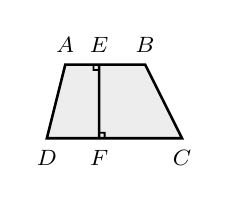
\begin{tikzpicture}[scale=0.39, baseline={(0,1.0)}, every node/.style={font=\footnotesize, text=black}]
    \coordinate (D) at (0,0); \coordinate (C) at (4.4,0);
    \coordinate (B) at (3.2,2.4); \coordinate (A) at (0.6,2.4);
    \coordinate (E) at (1.7,2.4); \coordinate (F) at (1.7,0);
    \fill[gray!14] (D)--(C)--(B)--(A)--cycle;
    \draw[black, line width=0.95pt] (D)--(C)--(B)--(A)--cycle (E)--(F);
    \rightbox[0.18cm]{A}{E}{F}\rightbox[0.18cm]{E}{F}{C}
    \node[above=1pt] at (A) {$A$}; \node[above=1pt] at (E) {$E$}; \node[above=1pt] at (B) {$B$};
    \node[below=1pt] at (D) {$D$}; \node[below=1pt] at (F) {$F$}; \node[below=1pt] at (C) {$C$};
  \end{tikzpicture}\par
  បាត៖ $AB$ និង \blank{1.0cm} $\;\vert\;$ កម្ពស់៖ \blank{1.1cm} &
  \centering
  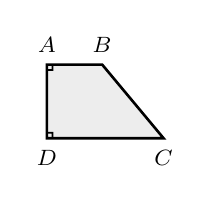
\begin{tikzpicture}[scale=0.39, baseline={(0,1.0)}, every node/.style={font=\footnotesize, text=black}]
    \coordinate (D) at (0,0); \coordinate (C) at (3.8,0);
    \coordinate (B) at (1.8,2.4); \coordinate (A) at (0,2.4);
    \fill[gray!14] (D)--(C)--(B)--(A)--cycle;
    \draw[black, line width=0.95pt] (D)--(C)--(B)--(A)--cycle;
    \rightbox[0.18cm]{B}{A}{D}\rightbox[0.18cm]{A}{D}{C}
    \node[above=1pt] at (A) {$A$}; \node[above=1pt] at (B) {$B$};
    \node[below=1pt] at (D) {$D$}; \node[below=1pt] at (C) {$C$};
  \end{tikzpicture}\par
  បាត៖ $AB$ និង \blank{1.0cm} $\;\vert\;$ កម្ពស់៖ \blank{1.1cm} &
  \centering\arraybackslash
  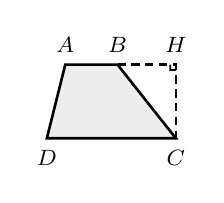
\begin{tikzpicture}[scale=0.39, baseline={(0,1.0)}, every node/.style={font=\footnotesize, text=black}]
    \coordinate (D) at (0,0); \coordinate (C) at (4.2,0);
    \coordinate (B) at (2.3,2.4); \coordinate (A) at (0.6,2.4); \coordinate (H) at (4.2,2.4);
    \fill[gray!14] (D)--(C)--(B)--(A)--cycle;
    \draw[black, line width=0.95pt] (D)--(C)--(B)--(A)--cycle;
    \draw[black, line width=0.8pt, densely dashed] (B)--(H)--(C);
    \rightbox[0.18cm]{B}{H}{C}
    \node[above=1pt] at (A) {$A$}; \node[above=1pt] at (B) {$B$}; \node[above=1pt] at (H) {$H$};
    \node[below=1pt] at (D) {$D$}; \node[below=1pt] at (C) {$C$};
  \end{tikzpicture}\par
  បាត៖ $AB$ និង \blank{1.0cm} $\;\vert\;$ កម្ពស់៖ \blank{1.1cm} \\[3pt]
  \hline
\end{tabular}

\vspace{4pt}
\begin{minipage}[c]{7.0cm}
  \centering
  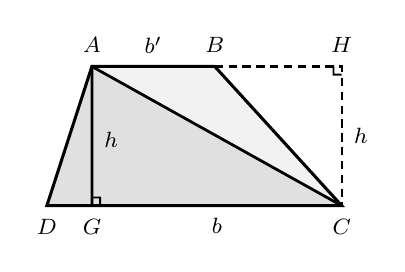
\begin{tikzpicture}[scale=0.52, every node/.style={font=\footnotesize, text=black}]
    \coordinate (D) at (0,0);
    \coordinate (G) at (1.1,0);
    \coordinate (C) at (7.2,0);
    \coordinate (A) at (1.1,3.4);
    \coordinate (B) at (4.1,3.4);
    \coordinate (H) at (7.2,3.4);
    \fill[gray!24] (D)--(C)--(A)--cycle;
    \fill[gray!10] (A)--(B)--(C)--cycle;
    \draw[black, line width=1.1pt] (D)--(C)--(B)--(A)--cycle;
    \draw[black, line width=1.0pt] (A)--(C) (A)--(G);
    \draw[black, line width=0.85pt, densely dashed] (B)--(H)--(C);
    \rightbox[0.20cm]{A}{G}{C}
    \rightbox[0.20cm]{B}{H}{C}
    \node[above=1.5pt] at (A) {$A$};
    \node[above=1.5pt] at (B) {$B$};
    \node[above=1.5pt] at (H) {$H$};
    \node[below=1.5pt] at (D) {$D$};
    \node[below=1.5pt] at (G) {$G$};
    \node[below=1.5pt] at (C) {$C$};
    \node[above=1pt] at (2.6,3.4) {$b'$};
    \node[below=1pt] at (4.15,0) {$b$};
    \node[right=1pt] at (1.1,1.6) {$h$};
    \node[right=1pt] at (7.2,1.7) {$h$};
  \end{tikzpicture}
\end{minipage}\hfill
\begin{minipage}[c]{11.5cm}
  \textbf{(ខ) រុករករូបមន្តតាមការពុះអង្កត់ទ្រូង $AC$ (ទំ.១៩២)៖}
  \begin{enumerate}[label=\enbf{\arabic*.}, leftmargin=1.4em, itemsep=2.5pt, topsep=1.5pt]
    \item អង្កត់ទ្រូង $AC$ ចែកចតុកោណព្នាយ $ABCD$ ជាត្រីកោណពីរ គឺ $\tri{ADC}$ និង $\tri{ABC}$៖
    \begin{itemize}[leftmargin=1.1em, itemsep=1.5pt, topsep=1pt]
      \item ផ្ទៃត្រីកោណ $\tri{ADC}$ (បាត $DC = b$, កម្ពស់ $AG = h$)៖ $S_{\tri{ADC}} = \dfrac{1}{2} \times$ \blank{0.9cm} $\times$ \blank{0.9cm}
      \item ផ្ទៃត្រីកោណ $\tri{ABC}$ (បាត $AB = b'$, កម្ពស់ក្រៅ $CH = h$)៖ $S_{\tri{ABC}} = \dfrac{1}{2} \times$ \blank{0.9cm} $\times$ \blank{0.9cm}
    \end{itemize}
    \item បូកផ្ទៃទាំងពីរ រួចដាក់ $\dfrac{1}{2}h$ ជាកត្តារួម៖\\
    $S_{ABCD} = S_{\tri{ADC}} + S_{\tri{ABC}} = \dfrac{1}{2}hb + \dfrac{1}{2}hb' = \dfrac{1}{2}($ \blank{1.9cm} $) \times h$។
    \item \textbf{វិនិច្ឆ័យកំហុសគំរូ៖} សិស្សម្នាក់គណនាផ្ទៃចតុកោណព្នាយ ($b=10, b'=6, h=4$) ដោយសរសេរ $S = 10 + 6 \times 4 \div 2 = 10 + 12 = 22$។ តើគាត់ខុសត្រង់ណា? ចម្លើយត្រឹមត្រូវស្មើប៉ុន្មាន?\\
    កំហុស៖ \blank{5.2cm} $\;\vert\;$ ចម្លើយត្រូវ $S =$ \blank{1.6cm}។
  \end{enumerate}
\end{minipage}

% ==================== ផ្នែកទី ៣ ៖ E3 - EXPLAIN ====================
\secbar{ផ្នែកទី ៣ ៖ សំយោគទ្រឹស្ដីបទ សម្រាយបញ្ជាក់ផ្លូវការ និងធនាគារហេតុផល (\enbf{E3 — Explain})}{\en{6} នាទី (ទំ.១៩១--១៩២)}

\begin{tcolorbox}[
  enhanced, sharp corners, colback=white, colframe=black,
  boxrule=1.0pt, boxsep=2pt, top=3.5pt, bottom=3.5pt, left=6pt, right=6pt
]
  $\bullet$ \textbf{ទ្រឹស្ដីបទ (ទំ.១៩១)៖} ផ្ទៃក្រឡាចតុកោណព្នាយដែលបាតមានរង្វាស់ $b,\; b'$ និងកម្ពស់កែង $h$ កំណត់ដោយរូបមន្ត៖ $\mathbf{S =}$ \blank{3.4cm} ។\\[2.5pt]
  $\bullet$ \textbf{សម្រាយបញ្ជាក់ផ្លូវការ (ទំ.១៩២)៖} ភ្ជាប់អង្កត់ទ្រូង $AC$ ហើយគូសកម្ពស់ $AG \perp DC$ និង $CH \perp AB$ ($AG = CH = h$)៖\\[2pt]
  \hspace*{0.3cm}$S_{ABCD} = S_{\tri{ADC}} + S_{\tri{ABC}} = \dfrac{1}{2} AG \cdot DC + \dfrac{1}{2} CH \cdot AB = \dfrac{1}{2} h \cdot$ \blank{1.0cm} $+ \dfrac{1}{2} h \cdot$ \blank{1.0cm} $= \dfrac{1}{2}($ \blank{1.8cm} $) \times h$។\\[4pt]
  \begin{tabular}{|p{4.4cm}|p{4.1cm}|p{4.2cm}|p{4.5cm}|}
    \hline
    \cellcolor{headgray}\centering\textbf{\cnum{1} លក្ខខណ្ឌបាត--កម្ពស់} &
    \cellcolor{headgray}\centering\textbf{\cnum{2} រូបមន្តផ្ទាល់} &
    \cellcolor{headgray}\centering\textbf{\cnum{3} រូបមន្តច្រាសរកកម្ពស់ $h$} &
    \cellcolor{headgray}\centering\arraybackslash\textbf{\cnum{4} រូបមន្តច្រាសរកបាត $b$} \\[2pt]
    \hline
    $b \parallel b'$ (បាតស្របទាំងពីរ) \par និង $h \perp b,\; h \perp b'$ &
    \centering $S = \dfrac{(b + b') \times h}{2}$ &
    \centering $h = \dfrac{2S}{b + b'}$ &
    \centering\arraybackslash $b + b' = \dfrac{2S}{h} \Rightarrow b = \dfrac{2S}{h} - b'$ \\[2pt]
    \hline
  \end{tabular}
\end{tcolorbox}

\newpage

% ==================== ទំព័រទី ២ ៖ E4, E5 និងកិច្ចការផ្ទះ ====================
\secbar{ផ្នែកទី ៤ ៖ លំហាត់គំរូតាមជំហាន (\enbf{E4 — Worked \& Faded Examples})}{\en{10} នាទី (ទំ.១៩២--១៩៣)}

\begin{tcolorbox}[
  enhanced, sharp corners, colback=white, colframe=black,
  boxrule=0.95pt, boxsep=2pt, top=3.5pt, bottom=3.5pt, left=6pt, right=6pt, after skip=4pt
]
  \textbf{លំហាត់គំរូទី ១ (ទំ.១៩២ — បិទបេសកកម្ម E1 ប្លង់ដីកសិដ្ឋាន $A$ និង $B$)៖} \textit{(សម្គាល់៖ រូបក្នុងផ្នែកទី១ មានបាតស្របឈរបញ្ឈរ!)}
  \begin{itemize}[leftmargin=1.2em, itemsep=2.5pt, topsep=2pt]
    \item \textbf{ប្លង់ដី $A$៖} បាតស្របបញ្ឈរ $b = 150\unit{m},\; b' = 126\unit{m}$ និងកម្ពស់កែង $h = 120\unit{m}$៖\\
    \hspace*{0.4cm}$S_A = \dfrac{(\blank{1.3cm} + \blank{1.3cm}) \times 120}{2} = \blank{1.4cm} \times 60 =$ \blank{2.2cm} $\unit{m}^2$។
    \item \textbf{ប្លង់ដី $B$៖} បាតស្របបញ្ឈរ $b = 100\unit{m},\; b' = 126\unit{m}$ និងកម្ពស់កែង $h = 130\unit{m}$៖\\
    \hspace*{0.4cm}$S_B = \dfrac{(\blank{1.3cm} + \blank{1.3cm}) \times 130}{2} = \blank{1.4cm} \times 65 =$ \blank{2.2cm} $\unit{m}^2$។
    \item \textbf{សន្និដ្ឋានបិទបេសកកម្ម E1៖} ប្លង់ដី \blank{0.9cm} ធំជាងប្លង់ដី \blank{0.9cm} ចំនួន $S_A - S_B =$ \blank{2.2cm} $\unit{m}^2$។
  \end{itemize}
\end{tcolorbox}

\begin{tcolorbox}[
  enhanced, sharp corners, colback=white, colframe=black,
  boxrule=0.95pt, boxsep=2pt, top=3.5pt, bottom=3.5pt, left=6pt, right=6pt, after skip=4pt
]
  \begin{minipage}[c]{12.3cm}
    \textbf{លំហាត់គំរូទី ២ (ទំ.១៩៣ — ច្រកចូលអគាររាងរូបសមាស)៖}\\
    ច្រកចូលនៃអគារមួយមានរាងជាចតុកោណកែង $CDEF$ បន្តុបចតុកោណព្នាយសមបាត $ABCF$ ពីលើដូចរូបខាងស្ដាំ។ គណនាផ្ទៃក្រឡានៃច្រកចូលអគារនោះ។
    \begin{itemize}[leftmargin=1.2em, itemsep=2.5pt, topsep=2pt]
      \item \textbf{ជំហានទី ១៖} បាតក្រោមនៃចតុកោណព្នាយ $ABCF$ គឺ $FC = ED =$ \blank{1.3cm} $\unit{m}$។\\
      ផ្ទៃចតុកោណព្នាយ៖ $S_{ABCF} = \dfrac{(6 + \blank{1.2cm}) \times 4}{2} =$ \blank{1.6cm} $\unit{m}^2$។
      \item \textbf{ជំហានទី ២៖} ផ្ទៃចតុកោណកែង $CDEF$៖ $S_{CDEF} = 8 \times 12 =$ \blank{1.6cm} $\unit{m}^2$។
      \item \textbf{ជំហានទី ៣៖} ផ្ទៃក្រឡាសរុប៖ $S = S_{ABCF} + S_{CDEF} =$ \blank{1.5cm} $+$ \blank{1.5cm} $=$ \blank{1.8cm} $\unit{m}^2$។
    \end{itemize}
  \end{minipage}\hfill
  \begin{minipage}[c]{5.8cm}
    \centering
    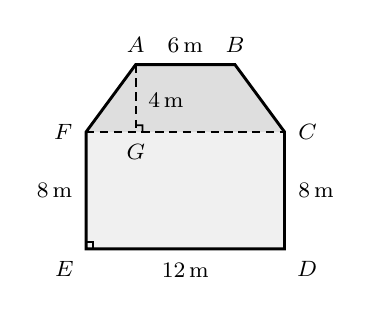
\begin{tikzpicture}[scale=0.45, every node/.style={font=\footnotesize, text=black}]
      \coordinate (E) at (0,0);
      \coordinate (D) at (5.6,0);
      \coordinate (C) at (5.6,3.3);
      \coordinate (F) at (0,3.3);
      \coordinate (G) at (1.4,3.3);
      \coordinate (A) at (1.4,5.2);
      \coordinate (B) at (4.2,5.2);
      \fill[gray!12] (E)--(D)--(C)--(F)--cycle;
      \fill[gray!26] (F)--(C)--(B)--(A)--cycle;
      \draw[black, line width=1.05pt] (E)--(D)--(C)--(B)--(A)--(F)--cycle;
      \draw[black, line width=0.85pt, densely dashed] (F)--(C) (A)--(G);
      \rightbox[0.19cm]{A}{G}{C}
      \rightbox[0.19cm]{F}{E}{D}
      \node[above=1pt] at (A) {$A$};
      \node[above=1pt] at (B) {$B$};
      \node[above=1pt] at (2.8,5.2) {$6\unit{m}$};
      \node[left=1.5pt] at (F) {$F$};
      \node[right=1.5pt] at (C) {$C$};
      \node[below=1pt] at (G) {$G$};
      \node[right=1pt] at (1.4,4.2) {$4\unit{m}$};
      \node[left=1.5pt] at (0,1.65) {$8\unit{m}$};
      \node[right=1.5pt] at (5.6,1.65) {$8\unit{m}$};
      \node[below left=1pt] at (E) {$E$};
      \node[below right=1pt] at (D) {$D$};
      \node[below=1.5pt] at (2.8,0) {$12\unit{m}$};
    \end{tikzpicture}
  \end{minipage}
\end{tcolorbox}

% ==================== ផ្នែកទី ៥ ៖ E5 - EVALUATE ====================
\secbar{ផ្នែកទី ៥ ៖ លំហាត់ប្រតិបត្តិ និងវាយតម្លៃរហ័ស (\enbf{E5 — Practice \& Exit Check})}{\en{10} នាទី (ទំ.១៩៣)}

\begin{minipage}[t]{8.6cm}
  \begin{tcolorbox}[
    enhanced, sharp corners, colback=white, colframe=black,
    boxrule=0.95pt, boxsep=2pt, top=3.5pt, bottom=3.5pt, left=5pt, right=5pt, equal height group=e5area3
  ]
    \textbf{ក. ប្រតិបត្តិ រូបទី១ (ទំ.១៩៣)៖} គណនាតម្លៃ $x$ បើ $S = 72\unit{cm}^2$៖
    \begin{center}
      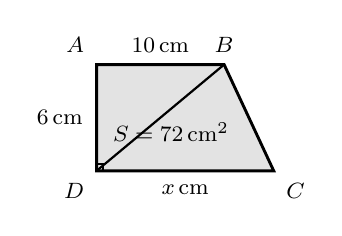
\begin{tikzpicture}[scale=0.45, every node/.style={font=\footnotesize, text=black}]
        \coordinate (D) at (0,0);
        \coordinate (C) at (5.0,0);
        \coordinate (B) at (3.6,3.0);
        \coordinate (A) at (0,3.0);
        \fill[gray!22] (D)--(C)--(B)--(A)--cycle;
        \draw[black, line width=1.05pt] (D)--(C)--(B)--(A)--cycle;
        \draw[black, line width=0.8pt] (D)--(B);
        \rightbox[0.19cm]{A}{D}{C}
        \node[above left=1pt] at (A) {$A$};
        \node[above=1pt] at (B) {$B$};
        \node[below right=1pt] at (C) {$C$};
        \node[below left=1pt] at (D) {$D$};
        \node[above=1pt] at (1.8,3.0) {$10\unit{cm}$};
        \node[left=1.5pt] at (0,1.5) {$6\unit{cm}$};
        \node[below=1.5pt] at (2.5,0) {$x\unit{cm}$};
        \node at (2.1,1.1) {$S=72\unit{cm}^2$};
      \end{tikzpicture}
    \end{center}
    តាម \cnum{4} ៖ $\dfrac{(10 + x) \times 6}{2} = 72$\\[2pt]
    $10 + x = \dfrac{2 \times 72}{6} =$ \blank{1.3cm} $\Rightarrow x =$ \blank{1.5cm} $\unit{cm}$។\\[3pt]
    \textbf{គ. តេស្តរហ័ស ៩០ វិនាទី (\en{Exit Check})៖} ចតុកោណព្នាយមានបាត $6\unit{cm},\; 10\unit{cm}$, កម្ពស់កែង $4\unit{cm}$ និងជ្រុងទ្រេត $5\unit{cm}$។ តើ $S = ?$\\[2pt]
    \chkbox\ \textbf{A.} $40\unit{cm}^2$ \hspace{1.2cm} \chkbox\ \textbf{B.} $32\unit{cm}^2$\\[2pt]
    \chkbox\ \textbf{C.} $26\unit{cm}^2$ \hspace{1.2cm} \chkbox\ \textbf{D.} $64\unit{cm}^2$
  \end{tcolorbox}
\end{minipage}\hfill
\begin{minipage}[t]{10.0cm}
  \begin{tcolorbox}[
    enhanced, sharp corners, colback=white, colframe=black,
    boxrule=0.95pt, boxsep=2pt, top=3.5pt, bottom=3.5pt, left=5pt, right=5pt, equal height group=e5area3
  ]
    \textbf{ខ. ប្រតិបត្តិ រូបទី២ (ទំ.១៩៣)៖} គណនាផ្ទៃក្រឡា និងបរិមាត្រនៃរូប៖
    \begin{center}
      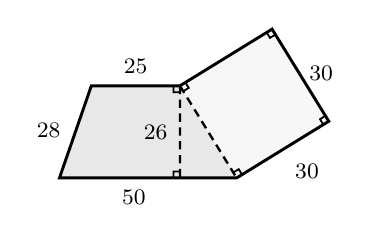
\begin{tikzpicture}[scale=0.45, every node/.style={font=\footnotesize, text=black}]
        \coordinate (P) at (0,0);
        \coordinate (Q) at (5.0,0);
        \coordinate (R) at (3.4,2.6);
        \coordinate (S) at (0.9,2.6);
        \coordinate (H) at (3.4,0);
        \coordinate (U) at ($(R)+(2.6,1.6)$);
        \coordinate (T) at ($(Q)+(2.6,1.6)$);
        \fill[gray!18] (P)--(Q)--(R)--(S)--cycle;
        \fill[gray!06] (Q)--(T)--(U)--(R)--cycle;
        \draw[black, line width=1.05pt] (P)--(Q)--(T)--(U)--(R)--(S)--cycle;
        \draw[black, line width=0.85pt, densely dashed] (R)--(H) (R)--(Q);
        \rightbox[0.18cm]{S}{R}{H}\rightbox[0.18cm]{R}{H}{P}
        \rightbox[0.18cm]{Q}{R}{U}\rightbox[0.18cm]{R}{U}{T}
        \rightbox[0.18cm]{U}{T}{Q}\rightbox[0.18cm]{T}{Q}{R}
        \node[above=1pt] at (2.15,2.6) {$25$};
        \node[below=1pt] at (2.1,0) {$50$};
        \node[left=1.5pt] at (0.42,1.35) {$28$};
        \node[left=1pt] at (3.4,1.3) {$26$};
        \node[below right=1pt] at (6.3,0.75) {$30$};
        \node[above right=1pt] at (6.7,2.4) {$30$};
      \end{tikzpicture}
    \end{center}
    $\bullet$ $S_{\text{ព្នាយ}} = \dfrac{(25 + 50)\times \blank{1.0cm}}{2} =$ \blank{1.5cm} $\;\vert\;$ $S_{\text{ការេ}} = 30\times 30 =$ \blank{1.4cm}\\[2pt]
    $\bullet$ ផ្ទៃក្រឡាសរុប $S =$ \blank{2.2cm} (មិនយកជ្រុងទ្រេត $28$ ទេ!)\\[2pt]
    $\bullet$ បរិមាត្រជុំវិញក្រៅ $P = 25 + 28 + 50 + 30 + 30 + 30 =$ \blank{1.6cm}\\[2pt]
    \chkbox\ \textit{បានផ្ទៀងផ្ទាត់ជាមួយដៃគូ (មិនបូកបន្ទាត់ភ្ជាប់ខាងក្នុងទេ!)}
  \end{tcolorbox}
\end{minipage}

% ==================== កិច្ចការផ្ទះ (ជំហានទី ៥) ====================
\vspace{3.5pt}
\begin{tcolorbox}[
  enhanced, sharp corners, colback=panelgray, colframe=black,
  boxrule=1.0pt, boxsep=2pt, top=3pt, bottom=3pt, left=6pt, right=6pt
]
  {\muol\fontsize{9.0pt}{13pt}\selectfont កិច្ចការផ្ទះ (សៀវភៅសិក្សាគោល ទំព័រ ១៩៤ — ធ្វើដាក់ក្នុងសៀវភៅលំហាត់សម្រាប់ម៉ោងក្រោយ)}\\[2pt]
  $\bullet$ \textbf{លំហាត់ទី ៣ (ទំ.១៩៤)៖} បំពេញតារាងចតុកោណព្នាយ៖ (ក) $b'=7\unit{cm}, b=11\unit{cm}, h=6\unit{cm} \Rightarrow S=?$ $\;\vert\;$ (ខ) $b'=8\unit{cm}, h=14\unit{cm}, S=126\unit{cm}^2 \Rightarrow b=?$ $\;\vert\;$ (គ) $b'=5\unit{cm}, h=8\unit{cm}, S=72\unit{cm}^2 \Rightarrow b=?$។\\
  $\bullet$ \textbf{លំហាត់ទី ២(រូបទី២) និងទី ៤ (ទំ.១៩៤)៖} រកកម្ពស់ $y$ ($b'=28\unit{cm}, b=38\unit{cm}, S=834\unit{cm}^2$) និងគណនា $AC, S_{ABCD}$ ក្នុងលំហាត់ទី៤។
\end{tcolorbox}

\end{document}
